\section{Country Avoidability Results}
\label{avoid_results}

\subsection{Brazil}

%\begin{figure}
%\centering
%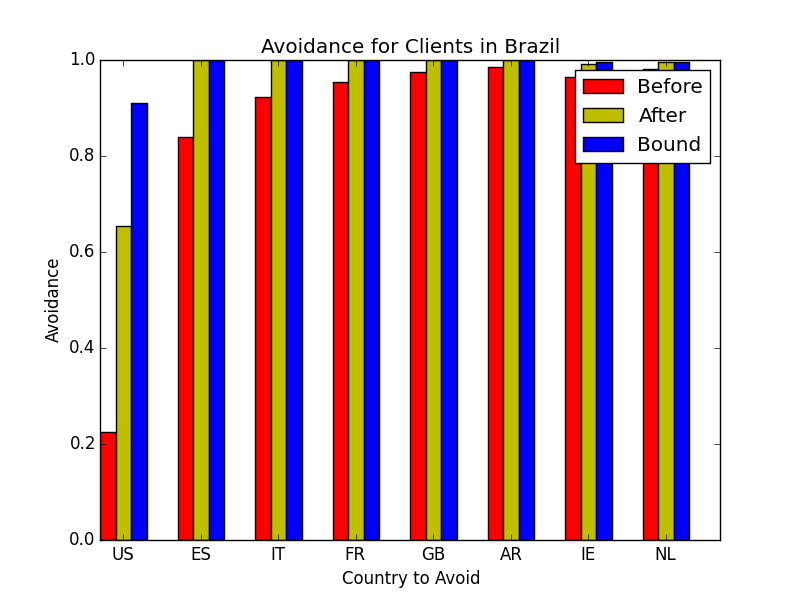
\includegraphics[width=.5\textwidth]{br_avoidance}
%\caption{A histogram of the number of third party requests are made by each initial domain request for the Brazilian Alexa Top 100 domains.}
%\label{fig:domains}
%\end{figure}

\subsection{Netherlands}

%\begin{figure}
%\centering
%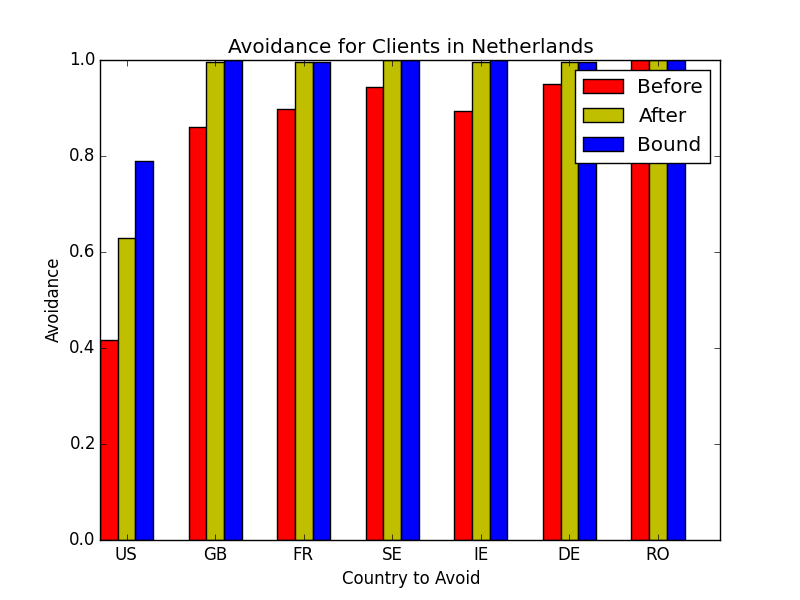
\includegraphics[width=.5\textwidth]{nl_avoidance}
%\caption{A histogram of the number of third party requests are made by each initial domain request for the Brazilian Alexa Top 100 domains.}
%\label{fig:domains}
%\end{figure}

\subsection{India}

%\begin{figure}
%\centering
%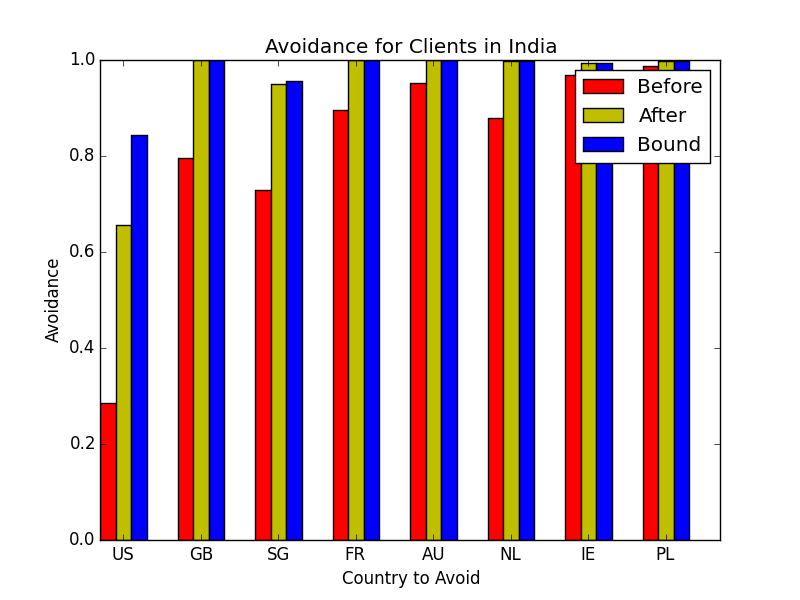
\includegraphics[width=.5\textwidth]{in_avoidance}
%\caption{A histogram of the number of third party requests are made by each initial domain request for the Brazilian Alexa Top 100 domains.}
%\label{fig:domains}
%\end{figure}

\subsection{Kenya}

%\begin{figure}
%\centering
%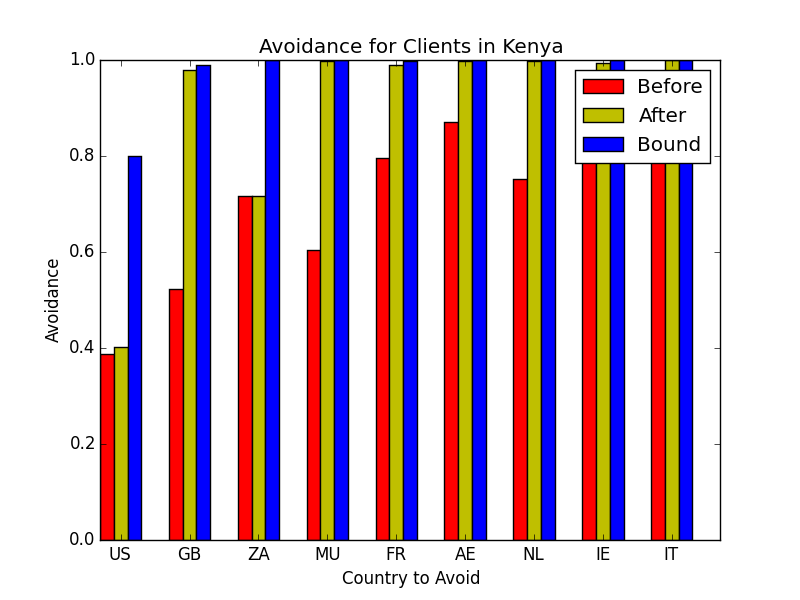
\includegraphics[width=.5\textwidth]{ke_avoidance}
%\caption{A histogram of the number of third party requests are made by each initial domain request for the Brazilian Alexa Top 100 domains.}
%\label{fig:domains}
%\end{figure}

\subsection{United States}

%\begin{figure}
%\centering
%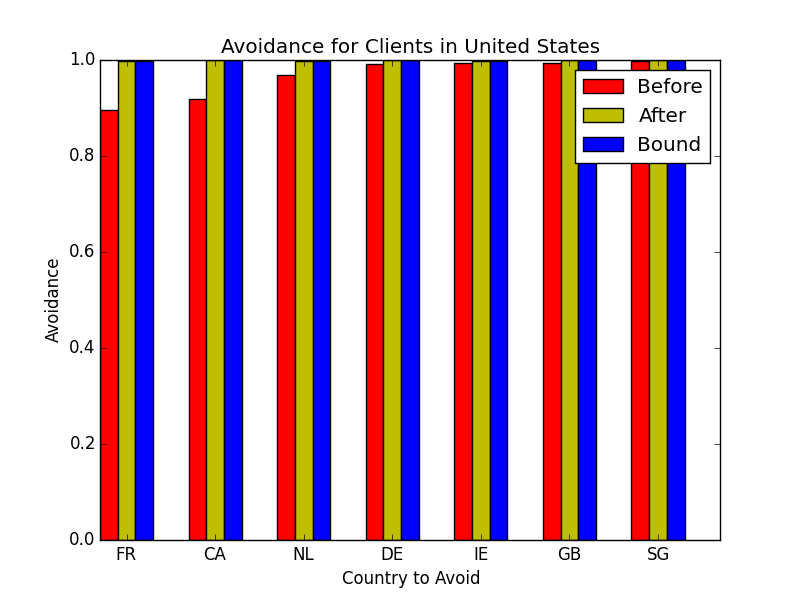
\includegraphics[width=.5\textwidth]{us_avoidance}
%\caption{A histogram of the number of third party requests are made by each initial domain request for the Brazilian Alexa Top 100 domains.}
%\label{fig:domains}
%\end{figure}

\subsection{Limitations}
\annie{discuss latency issues here}
